\documentclass[12pt,letterpaper]{article}
\usepackage[utf8]{inputenc}
\usepackage{kpfonts}
\usepackage[T1]{fontenc}

% custom titles
\usepackage{titlesec}

% fix broken title numbering with 2016 titlesec update
\usepackage{etoolbox}

\makeatletter
\patchcmd{\ttlh@hang}{\parindent\z@}{\parindent\z@\leavevmode}{}{}
\patchcmd{\ttlh@hang}{\noindent}{}{}{}
\makeatother
%%%

\titlespacing*\section{0pt}{12pt plus 4pt minus 2pt}{0pt plus 2pt minus 2pt}
\titlespacing*\subsection{0pt}{12pt plus 4pt minus 2pt}{0pt plus 2pt minus 2pt}
\titlespacing*\subsubsection{0pt}{12pt plus 4pt minus 2pt}{0pt plus 2pt minus 2pt}

% Package for double spacing
\usepackage{setspace}
\usepackage{ragged2e}

% Set 1.0 inch margins
\usepackage[margin=1.0in, headheight=15pt]{geometry}
\usepackage{enumitem}

% Use images and graphics
\usepackage{graphicx}
\usepackage{float}

% Use nicer headers
\usepackage{fancyhdr}
\pagestyle{fancy}
\renewcommand{\headrulewidth}{0pt}
\rhead{CIS3750 - Lab Demo 2}

% sections should be indexed with alphabets
\renewcommand{\thesection}{\Alph{section}}

%double spaced lines in the whole document
\doublespacing

\title{Assignment 1}

\begin{document}
\begin{titlepage}
    \centering
    \vspace*{\baselineskip}
    \rule{\textwidth}{1.6pt}\vspace*{-\baselineskip}\vspace*{2pt}
    \rule{\textwidth}{0.4pt}\\[1.5\baselineskip]
    {\LARGE \textsc{Reflections on a Wireframing Session}}\\[\baselineskip]
	\rule{\textwidth}{0.4pt}\vspace*{-\baselineskip}\vspace{4pt}    
    \rule{\textwidth}{2pt}\\[2\baselineskip]
   
    \vspace*{5\baselineskip}
    \textsc{BY}\\[0.25\baselineskip]
    {\LARGE HANLON} \\
    
    \vspace*{\baselineskip}
    % List of authors in alphabetical order (by last name)
    {\textsc{David DiMaria \\ Braydon Johnson \\ Joshua Lemieux \\ Neivin Mathew \\ Like Zheng} \par}
    \vfill
    {\scshape November 16, 2016} \\
  \end{titlepage}
  
  
% Table of Contents (no page numbers on contents)
\pagenumbering{roman} %roman numerals for ToC
\tableofcontents
\lhead{} % remove default header from Contents page
\clearpage
\pagenumbering{arabic} %pagenumbering in arabic numbers
    
\clearpage
\section{Wireframing Prototyping Session}
The Wireframing Prototyping Session was completed on November 9, 2016 during the scheduled lab time.
\section{Team Details}
\subsection{Team Name}
The team name for the project is "Hanlon."\par
The name is inspired by the eponymous highway that runs through the city of Guelph, and signifies the team's ties to the University of Guelph, and its beautiful city.\\

\begin{figure}[H]
	\centering	
	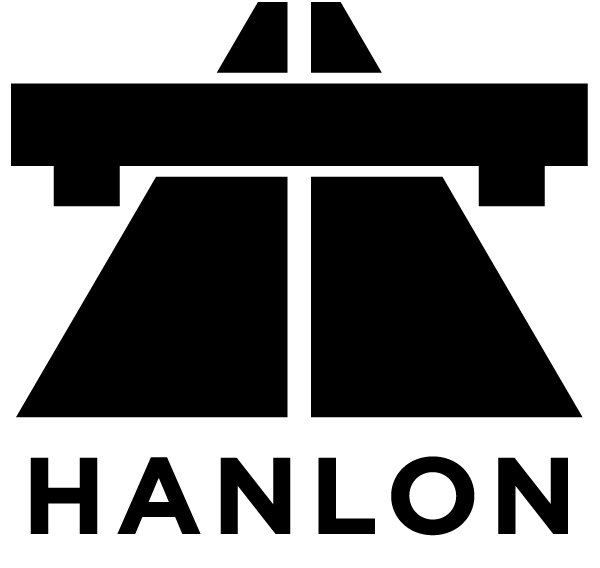
\includegraphics[height=2in]{img/hanlon-logo.png}
	%\caption{The team logo}
	\label{fig:kitten}
\end{figure}

\subsection{Team Members}
Hanlon is comprised of the following students:\\
1. \textbf{\hspace*{8pt}David DiMaria} - Project Manager\\
2. \textbf{\hspace*{8pt}Braydon Johnson} - Software Developer, User Interface Designer\\
3. \textbf{\hspace*{8pt}Joshua Lemieux} - Project Manager, User Interface Designer\\
4. \textbf{\hspace*{8pt}Neivin Mathew} - Software Developer, User Interface Designer\\
5. \textbf{\hspace*{8pt}Like Zheng} - Software Developer

\subsection{Team Roles}
\subsubsection*{Project Manager}
The Project Manager predicts potential problems that may arise during development, and plans tasks to ensure that the project is completed successfully and on time. This role involves the scheduling and unblocking of tasks. It may also involve some programming.

\subsubsection*{Software Developer}
The Developer is involved in all aspects of the software development process including research, design, coding, documentation and testing.

\subsubsection*{User Interface Designer}
The User Interface (UI) Designer role is to plan out and develop any user facing component of the system which includes the specific layout of screens, and improving the interaction between the customer and the product.

\subsection{Prototyping Session Roles}
The members of Hanlon were responsible for different aspects of the prototyping session:\\
1. \textbf{\hspace*{8pt}David DiMaria} - Facilitator\\
2. \textbf{\hspace*{8pt}Braydon Johnson} - Observer/Note Taker\\
3. \textbf{\hspace*{8pt}Joshua Lemieux} - Human Computer\\
4. \textbf{\hspace*{8pt}Neivin Mathew} - Observer/Note Taker\\
5. \textbf{\hspace*{8pt}Like Zheng} - Observer/Note Taker

\subsection{Team Organization}
Hanlon will follow a static team structure. Each member will maintain their respective roles for the entire duration of the project. \par

Hanlon will use a democratic majority voting system for any decisions that need to be taken within the team. Each present member will be involved in voting, and possesses one vote per motion. A motion is passed when a simple majority is achieved. \par

In the event of a team member being unavailable, and a majority cannot be established, a motion can only be passed through unanimous consent.

\clearpage
\section{Client Details and Use Cases}
\subsection{List of Use Cases}
Participants of the Paper Prototyping session were presented with the following use cases:\\
1.\hspace*{8pt} Create a Farmer user account\\
2.\hspace*{8pt} Login to a Farmer user account\\
3.\hspace*{8pt} Answer an ARET Survey\\
4.\hspace*{8pt} Download a Research Article\\
5.\hspace*{8pt} Add a crop to your list of Crops\\
6.\hspace*{8pt} Harvest one of your Crops\\
7.\hspace*{8pt} Delete one of your Crops\\
8.\hspace*{8pt} Change your name in your User Profile\\
9.\hspace*{8pt} Change your Account Password\\
10.\hspace*{3pt} Log out of your Farmer user account


\subsection{Participants}
The prototyping session included the following three participants:\\
1.\hspace*{8pt} \textbf{Corey Alexander}\\
Corey is a Teaching Assistant (TA) in his late twenties. He worked through only five of our use cases because he had a lot of feedback to give. He completed use cases 1, 2, 3, 9, and 10. He did have an issue when working through our use cases that involved editing the user's profile. He was confused by some of our button placements and felt there was some inconsistency with the rest of the application. This issue however was specific to the edit name and edit password use cases. Corey appeared to be moderately proficient with computers and was generally familiar with mobile applications.\\[0.5\baselineskip]
3.\hspace*{8pt} \textbf{Oliver Cook}\\
Oliver is a Teaching Assistant (TA) in his mid twenties, who is proficient with computers and is not representative of the client. He completed all of the use cases quite rapidly, and generally felt that the wireframe prototype behaved exactly as he expected it to. He was confused by the "Edit Profile" screen, and felt that the application was forcing him to change every single field in his profile.\\[0.5\baselineskip]
2.\hspace*{8pt} \textbf{Iranaeus Chan}\\
Iranaeus is an Zoology research student in his mid twenties. He was able to complete every use case except for the last two. He had an issue with the naming of the “Harvest” button in the "Harvest one of your Crops" use case. He felt that the button wasn’t indicative of what the Harvest page is meant for and was misleading. He felt that it meant someone would harvest the crops for him. Iranaeus seemed to be quite proficient with computers and was also familiar with mobile applications and their design.\\[0.5\baselineskip]

\clearpage
\section{Things That Worked}
Overall, the response to our wireframe was overwhelmingly positive. It was difficult to evaluate exactly what elements of our design worked well since participants would not notice things that were as they expected. Thus, we can assume that any element of the design that the participants did not have trouble with was well designed and behaved in a way that was expected. However, we received many comments about how intuitive many of the use cases were to accomplish. All of our participants went through most use cases without any help or difficulty.\par 
All participants thought that the process of login, and account creation went exactly as they expected. They felt that the process was straightforward, and agreed that the flow was intuitive. Upon reaching the home screen, all participants were able to recognize the menu bar at the bottom of their screen and identified it as the primary means of navigating through the application. There was no confusion of how to navigate the menu bar with a few changes made to the appearance of the menu bar. \par
The process of adding new crops to the list of the user's currently growing crops seemed to be well received by all the participants. Most participants felt the add button occupied the same section of the screen that they expected it to be in and were able to successfully search for a new crop and add it to their growing crops without any hassles.\par
All participants agreed that new surveys available to them on their home screen were appropriately positioned and visible enough to catch their attention without being obtrusive to other application functionality. Participants also found the ability to answer a survey simple and intuitive. \par

\clearpage
\section{Things to Improve}
Although most participants were able to easily navigate through the system without much trouble, there were some aspects of the design that were found wanting.\par
One of our participants wanted a header bar for the Login screen. Currently there is no indication at the top of the page that the user is on the sign-in screen. This can be easily implemented in a future release by adding a header bar that is consistent with the rest of the application.\par
All our participants were able to successfully change their password, but were not provided with any feedback indicating whether their password was changed successfully or not. The user did not have any information as to whether the application had done what they had wanted it to do or not. Adding a pop-up notification that informs the user of this would easily resolve this issue.\par
 	One participant was confused about the edit profile page. They felt like the page required the user to change everything in their profile instead of a single field. In the final version of the app the profile screen will auto populate the fields to indicate that you do not have to edit all fields to make a change.\par
	Another participant felt like the change password button was misleading. They felt like it looked like a submit button and was placed where a submit button would be placed. For future releases we will change the button to be a text link to avoid confusion.\par


\clearpage
\section{Looking to the Future}
Throughout the prototyping session, the participants made a number of suggestions about improvements that they would like to see to some features of the application. Some also wished that there were additional features for certain parts of the application.\par	
One participant thought it would be useful to have a harvest history within the harvest page. This is something that we are going to put in the final application, with a “last time harvested” label when you view each crop you’re growing. We also plan on putting a full crop history in the profile tab, with each crop you add, deleted or harvested.\par
	Some users felt that the buttons and interface may have been difficult to see for colourblind users. Our colour scheme had a contrast ratio of 4:1, just missing the recommended 4.5:1 contrast ratio. We do not have a final colour scheme, and this is something we would take into consideration in our final design.Simply using a slightly darker version of the green we had chosen, would fix this issue instantly.\par
	One user did not like the fact that the crop was added when clicking on a crop that you have searched for. They felt like when tapping on the crop a page should pop up with more information about that crop. This is a change we would like to make in the future. When tapping on a crop a page will open up that will show more information about that crop as well as a add and cancel button. This will allows users to get information about a crop before adding it.\par
Some users felt a bit lost with all the different screens that were available to them and wished that there was something to guide them within the application itself. The addition of a tutorial section which would execute for the first run of the application would resolve this issue and would not be difficult to maintain or implement. It would also vastly improve the usability of the application.\par
Some users wished that there was a better way to sort the research articles displayed within the research section of the application. They felt that simply searching for keywords within articles was not enough and wanted a way to browse through the articles without knowing what they were looking for. Adding functionality to browse through research articles by date, tags, category, author, or crop would help resolve this need. Allowing users to see what research articles have been viewed the most or used the most would also help them choose which article would be helpful to them. This functionality would not be difficult to implement as it would require fetching slightly more specific data and would also be straightforward to maintain.\par

\clearpage
\section{Individual Contributions}
\subsection{David DiMaria}
\textbf{Yes! And... Using Improv}\par
Considering I was the facilitator, and I chose to go without a script, I had to use some of the improv skills that we learned in class from The Making Box. First of all I had to make eye contact when explaining the purpose of our app and what paper prototyping is. This was a helpful skill because I needed to make sure they understood how to paper prototype, and maintaining eye contact makes it easier for them to listen to what I was saying.\par
One of the skills that I actually couldn’t use was the Yes, And… skill. The reason for this is when a participant asked for clarification on a use case, I wasn’t allowed to lead them in the right direction. As much as I wanted to lead them in the right direction with a new idea, it would have made it more difficult to determine if the system was intuitive to them. Also I explicitly wasn’t allowed to give suggestions in the paper prototype session, so I had to abandon the Yes, And… tactic for the morning. 


\clearpage
\subsection{Braydon Johnson}
\textbf{The Yes! And... Lab Demo}\par
During the lab demo I did not use any of the skills from the Yes! And… philosophy, this was because I was a note taker and did not interact with the participants at all. Honestly, I don’t believe the skills would have been that useful, previously when I talked about it they were helpful because they gave us the tools to build on other people’s ideas rather than shut them down in place of our own ideas.\par
In the prototyping session it was mostly watching and listening to the client, which certainly limited the options of techniques to use especially for those of us who had no real reason to interact with the participant. While there are some tools that promote our listening skills I previously stated that I wasn’t very fond of First Letter Last Letter as it made it too hard to focus on what they were saying as a whole because I was too busy listening for the end of their sentence. 

\clearpage
\subsection{Josh Lemieux}
\textbf{Yes!And...Lab Demo}\par
For our paper prototyping session, I personally did not use any of the techniques as I was the Human Computer (Beep Boop). I was not allowed to communicate with the client. I was only there to provide smooth transitions between screens following the client's’ input. There were times where my group members used a little bit of knowledge gained during the prototyping session though.\par
	The last client had some rather odd suggestions that were not typical in mobile applications. Rather than immediately shutting the idea down we thought about how that would be implemented and work in our app. It turns out that they just didn’t work out with our app, but that’s okay! By taking that time to review a suggestion that initially seems to not fit with our application, we may come to see that an odd suggestion could add benefit to our application.\par
      	A lot that we learned in the improv session is not exactly applicable to the paper prototyping session. This is because you are supposed to keep your interactions with the client to be as limited as possible. This is to get their “natural” reaction to using the application. I can see us using these techniques for our wire framing session when we are communicating more directly with the client.


\clearpage
\subsection{Neivin Mathew}
\textbf{Improv and Open-Mindedness}\par
It was rather difficult to completely apply the techniques I learned during the Improv session during the wireframing session, mostly because I was simply observing the participants of the prototyping session and taking notes detailing their interaction with the application model.\par
However, even though I did not directly interact with anyone during the session, the principles behind the "Yes!And..." philosophy did help me analyze the prototype more critically.\par 
It is easy to get invested in something when you have worked on it for a long time. You begin to look at your brainchild through rose coloured glasses and often remain oblivious to glaring errors in design. It's very hard to even accept criticism for your work, especially after you have spent hundreds of hours perfecting it. \par
However, the methods I learned in the Improv session definitely helped me keep an open mind about our design and forced me to be more flexible about possible changes. Accepting every change suggested by the user really opened my eyes to some design flaws that I would not have seen otherwise. For example, I was under the impression that our colour scheme was appropriately chosen and was perfectly readable. I was sorely mistaken, since one of our participants pointed out that our colour scheme did not pass the recommended 4.5:1 contrast ratio test for readability. Remembering the methodology of "Yes!And..." really helped me realize the importance of considering different perspectives in design, especially that of a potential user. 

		
	
\clearpage
\subsection{Like Zheng}
\textbf{Yes!And... Philosophy}\par
During the prototyping session, my role was that of observer and note taker. I was responsible for observing the user's behaviour, taking notes about how the system performs, and how the user responds as well.\par
Thus, it was not my job to talk to the participant. However, our facilitator was responsible for that. I noticed that the way our facilitator communicated with participant was much more listening than talking. This is important to minimize any influence our words would have on the participant, and allow them to give us their unbiased opinion. They can now give us a true reflection of what they are thinking.\par 
The “Yes! And… philosophy was not useful during prototyping session. It is a tool for changing ideas, and in prototyping session, we were listening to the user's ideas for most of the time. Thus, I did not find the technique helpful for the prototyping session. 

\end{document}